\chapter{Projekt serwisu}
\thispagestyle{chapterBeginStyle}

W tym rozdziale przedstawiono opis projektu systemu w notacji UML uwzględniający wymagania funkcjonalne opisane we wstępie. Do opisu relacji pomiędzy składowymi systemu wykorzystano diagramy UML.

\section{Struktura}

W serwisie wykorzystano architekturę klient-serwer. Istnieje jeden serwer, do którego może podłączać się wiele klientów i odpowiada on za komunikację i zarządzanie danymi.
W komponencie klienta wykorzystano architekturę trójwarstwową. Architektura ta dzieli komponent na trzy osobne części:
\begin{itemize}
	\item warstwa prezentacji,
	\item warstwa biznesowa,
	\item warstwa danych.
\end{itemize}
Warstwa prezentacji jest to interfejs graficzny użytkownika. Jest odpowiedzialna za interakcję z użytkownikiem (wyświetlanie i wprowadzanie danych). \\ \\
Warstwa biznesowa odpowiada za przetwarzanie komunikatów od użytkownika lub ze strony serwera. Tutaj zawarta jest wszelka logika aplikacji. Przetworzone dane są przekazywane do warstwy prezentacji i/lub warstwy danych. Warstwa ta jest łącznikiem pomiędzy warstwą prezentacji, a warstwą danych. \\ \\
Warstwa danych jest dostępem do danych. Obsługuje połączenie aplikacji z zewnętrznym obiektem dostarczającym dane (baza danych, serwer). \\ \\ \\ \\ \\ \\ \\ \\ \\ \\ \\ \\ \\ 

\section{Przypadki użycia}
Poniżej został przedstawiony diagram ukazujący możliwe przypadki użycia występujące w serwisie.

\begin{figure}[h!]
	\begin{center}
		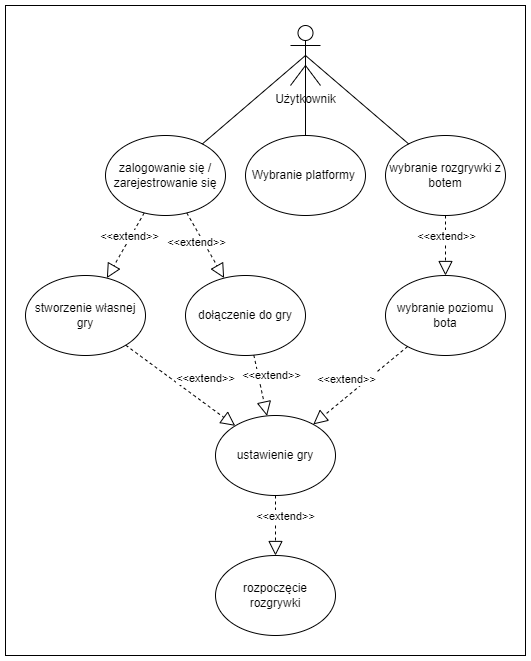
\includegraphics[width=10cm,height=12cm]{img/przypadki-uzycia.png}
	\end{center}
	\caption{{\color{dgray} Diagram przypadków użycia.}} 
	\label{przypadki_uzycia}
\end{figure} 

Użytkownik może wybrać na jakiej platformie będzie chciał korzystać z serwisu. Ma do wyboru stronę internetową albo aplikacje na telefon. Aby móc dołączyć do gry z innymi graczami należy zalogować się lub zarejestrować w aplikacji. Następnie gracz ma możliwość stworzenia własnej gry lub dołączenia do innej. Jeśli zdecyduje się stworzyć własną grę, musi wybrać od 2 do 4 osób spośród wszystkich aktywnych graczy. Panel konfiguracji gry umożliwia zadeklarowanie dozwolonego czasu na wykonanie ruchu oraz liczbę graczy. Dołączenie do innej gry działa na zasadzie znalezienia oczekującej gry o takich samych ustawieniach, jakie wprowadził gracz, albo poprzez otrzymanie zaproszenia od innego użytkownika. Jeśli wszystkie miejsca w grze zostały wypełnione rozgrywka się rozpoczyna. W przypadku wybrania gry z botem, odbywa się ona lokalnie bez łączenia z serwerem. Użytkownik ma do dyspozycji dwa poziomy bota. Następnie również konfiguruje grę i rozpoczyna rozgrywkę. \\ \\ \\ \\

\section{Diagramy aktywności}

W tym podrozdziale zostały przedstawione dwa diagramy aktywności skupiające się na przebiegu głównych funkcjonalności aplikacji.

\begin{figure}[h!]
	\begin{center}
		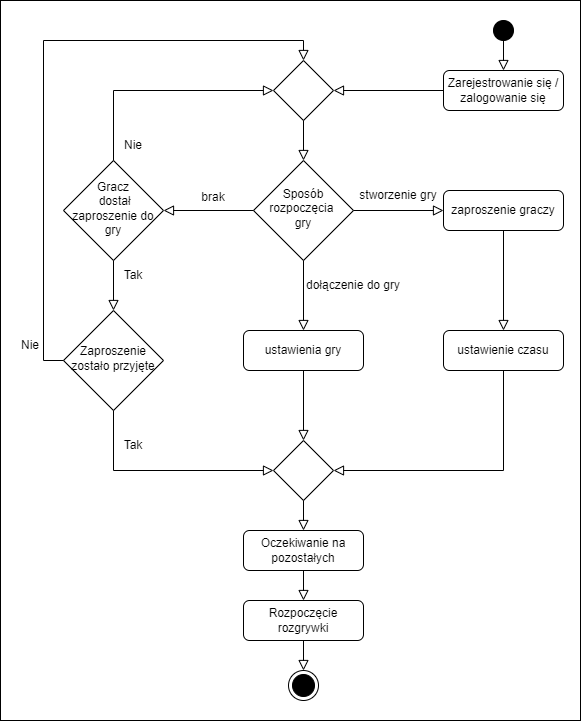
\includegraphics[width=10cm,height=12cm]{img/activity-diagram-start-game.png}
	\end{center}
	\caption{{\color{dgray} Diagram aktywności rozpoczęcie gry.}} 
	\label{diagram-aktywnosci-start}
\end{figure}

Powyższy diagram ukazuje proces przebiegu rozpoczęcia gry z innymi użytkownikami. Aby móc rozpocząć rozgrywkę z graczami trzeba posiadać konto, a więc proces rozpoczyna się od zarejestrowania się bądź zalogowania się. Następnie gracz może wybrać sposób w jaki przystąpi do rozgrywki. Ma możliwość stworzenia własnej gry i zaproszenia poszczególnych dostępnych użytkowników. Po wybraniu graczy deklaruje czas przeznaczony na ruch w grze. Drugą opcją jest dołączenie do pierwszej znalezionej gry o takiej samej konfiguracji jaką zadeklarował użytkownik i która nadal oczekuje na dołączenie innych graczy. W przypadku nieznalezienia takiej rozgrywki gracz jest dołączany do nowo utworzonej gry o podanych parametrach. Jeśli jednak tego nie zrobi, może oczekiwać na zaproszenie od innego użytkownika. Po pojawieniu się takiego zaproszenia ma możliwość przyjęcia go lub odrzucenia. Jeśli zaakceptuje to jest dołączany do gry z ustawieniami narzuconymi przez zapraszającego. Bez względu na to jaką opcje rozpoczęcia gry gracz wybierze, to w następnym kroku oczekuje, aż do gry dołączą wszyscy wymagani gracze. Proces kończy się rozpoczęciem rozgrywki. \\ \\ \\ \\ \\

\begin{figure}[h!]
	\begin{center}
		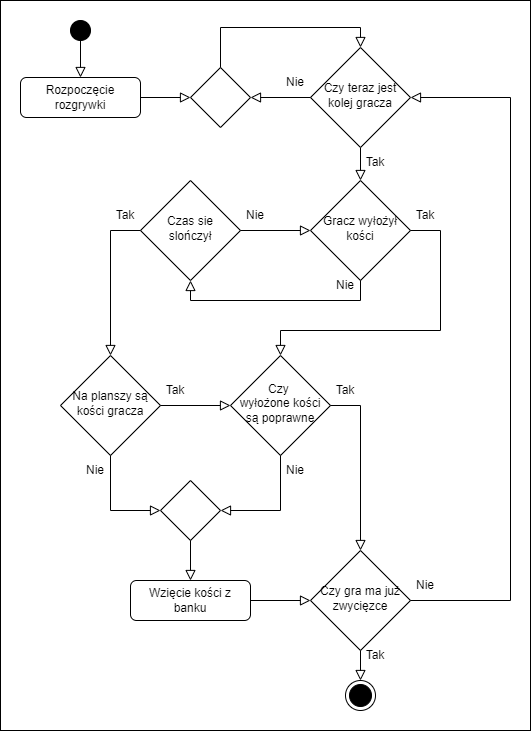
\includegraphics[width=10cm,height=12cm]{img/activity-diagram-game.png}
	\end{center}
	\caption{{\color{dgray} Diagram aktywności rozgrywki.}} 
	\label{diagram-aktywnosci-game}
\end{figure}  

Diagram ukazany na rysunku powyżej ukazuje proces przebiegu rozgrywki. Użytkownik oczekuje na własną kolej ruchu. W sytuacji, gdy po wykonaniu ruchu przez innego gracza, jest wyłaniany zwycięzca, gra dobiega końca. Natomiast jeśli następuje kolej gracza, ma on możliwość modyfikowania planszy i wykładaniu własnych kości. Na wykonanie ruchu każdy gracz ma określoną ilość czasu zadeklarowaną w trakcie tworzenia gry. Wyłożenie kości oznacza, że gracz zatwierdza modyfikacje przeprowadzone na planszy. Następnie zmiany dokonane na planszy są weryfikowane pod względem poprawności z zasadami gry. W przypadku, gdy czas upłynął zanim gracz potwierdził ruch, sprawdza się, czy na planszy znajdują się kości wyłożone przez gracza. Jeśli ich nie ma, gracz otrzymuje jedną kość z puli wolnych kości. Jeśli jednak na planszy znajdują się jakieś kości gracza, to zmodyfikowane zbiory kości są również weryfikowane pod względem poprawności. W przypadku niespełnienia zasad gry gracz otrzymuje nową kość. 
Jeśli gracz wyłożył wszystkie swoje kości, bądź wziął z banku ostatnią kość, gra dobiega końca.


